\documentclass[10pt]{article}
\usepackage[margin=1in]{geometry}
\usepackage[T1]{fontenc}
\usepackage{lmodern}
\usepackage{amsmath,amssymb}
\usepackage{booktabs}
\usepackage{graphicx}
\usepackage{caption}
\usepackage{xcolor}
\usepackage[numbers,sort&compress]{natbib}
\usepackage[colorlinks=true,linkcolor=blue!50!black,citecolor=blue!50!black,urlcolor=blue!50!black]{hyperref}
\captionsetup{font=small,labelfont=bf}
\graphicspath{{figures/}}

\title{Does Evidence-Aware Trust Calibration Help?\\
\large A Reproduction and Simulation Study of Adaptive Trust Cues for Autonomous Research Agents}
\author{Mili Acharya\\ Indian Institute of Information Technology Allahabad\\ \texttt{mhm2026006@iiita.ac.in}}
\date{November 2026}

\begin{document}
\maketitle

\begin{abstract}
Autonomous research agents retrieve, extract, summarise and synthesise evidence with reliability that varies across pipeline stages and across the evidence behind each claim. Existing trust-calibration cues, however, operate at the level of the agent or the situation. Building on a prior literature review that proposed an evidence-aware calibration framework, we (i) re-implement the adaptive trust-calibration cue (TCC) of Okamura and Yamada from its published description and test whether its qualitative effect reproduces in a simulated replica of the original protocol, and (ii) extend the comparison to a simulated autonomous-research pipeline in which the ground-truth probability that each claim is correct is known. Across 50 paired seeds with simulated users, a per-claim, evidence-aware warranted-trust cue reduced expected decision cost by 10.8\% relative to no cue and by 5.9\% relative to the adaptive TCC (Holm-corrected paired Wilcoxon, $p<0.001$), and lowered trust-calibration error by 0.042--0.045. Against the TCC, however, the gain came entirely from fewer needless verifications: the rate of accepted wrong claims did not differ ($p=0.18$). The advantage vanished when evidence carried no information about correctness, and when simulated users rarely followed cues. It persisted after a mid-session drop in agent reliability. The reproduction recovered the original study's main effect (more manual choices after reliability drops) but not its null effect on accuracy, a discrepancy we attribute to the absence of time pressure in the simulation. Because all users are simulated, the results establish mechanisms and boundary conditions, not human effect sizes.
\end{abstract}

\section{Introduction}
Humans who supervise AI agents should rely on them neither more nor less than the agents warrant~\cite{mehrotra2024systematic,wischnewski2023measuring}. The author's earlier review~\cite{acharya2026review} traced how calibration research has moved from reliability- and transparency-based approaches~\cite{chen2018situation,akash2020human} to adaptive cues~\cite{okamura2020adaptive,okamura2020empirical} and mutual adaptation~\cite{devisser2020longitudinal}. It argued that autonomous research poses a particular problem: one agent may be highly reliable at retrieving sources yet unreliable at synthesising conflicting results, and every claim it produces rests on evidence of different quality. In the review's terms, \emph{agent reliability $\neq$ evidence quality}, and warranted trust should be estimated per claim. The review identified this \emph{evidence-aware calibration} gap (its \S8.2) and proposed a framework without testing it.

This paper turns that proposal into a controlled, reproducible experiment. We follow the reproduction-plus-extension pathway. First, we re-implement a published, well-specified adaptive calibration mechanism, the trust calibration cue (TCC) of Okamura and Yamada~\cite{okamura2020adaptive}, and check that it behaves as reported. Second, we use it as a baseline in a simulated autonomous-research pipeline where ground truth is known, and compare it with an evidence-aware cue derived from the review's framework.

\paragraph{Research questions.}
\textbf{RQ1} (reproduction): does the re-implemented TCC reproduce the original study's qualitative findings in a simulated replica of its protocol?
\textbf{RQ2} (extension): does an evidence-aware, per-claim cue lower decision cost and calibration error relative to (B0) no cue, (B1) an agent-level reliability display and (B2) the adaptive TCC?
\textbf{RQ3} (limits): under which conditions does any advantage disappear?

\paragraph{Contributions.} (1) An open, tested re-implementation of the TCC detection rule, with a documented partial reproduction. (2) A paired-seed simulation benchmark for trust calibration in research pipelines with known warranted trust. (3) Evidence that per-claim cues help mainly by reducing \emph{under}-reliance relative to an over-trust-only cue, together with three boundary conditions under which they do not help. We do not claim a new algorithm, and we make no claim about human effect sizes.

\section{Background and Related Work}
\paragraph{Calibration and warranted trust.} Following the review, we write calibration error as $E_{trust}=|T_{human}-T_{warranted}|$, where $T_{warranted}$ is the trust that the evidence and the agent's reliability justify~\cite{acharya2026review}. Surveys note that measures of appropriate trust are heterogeneous and that behavioural (reliance-based) measures are needed alongside self-report~\cite{wischnewski2023measuring,mehrotra2024systematic}. We therefore use behavioural metrics only.

\paragraph{Transparency.} Situation-awareness-based transparency exposes an agent's state and reliability to its user~\cite{chen2018situation}; Akash et al.\ vary transparency dynamically according to estimated trust and workload~\cite{akash2020human}. Our B1 is a deliberately simple instance: a continuously displayed estimate of agent-level reliability.

\paragraph{Adaptive trust calibration.} Okamura and Yamada infer trust from behaviour: choosing the automatic option signals that trust exceeds self-confidence~\cite{okamura2020adaptive}. A checkpoint is flagged as over-trust when the user chooses automation although manual success probability exceeds the automation's reliability; a cue fires when the current checkpoint and at least one of the two preceding checkpoints are flagged. In an online drone-inspection study (30 checkpoints, automation 90\% reliable until a storm after checkpoint 6, then 50\%), TCC groups increased manual choices in bad weather while the no-TCC group did not, and accuracy did not differ significantly~\cite{okamura2020adaptive}. A follow-up found that adaptive TCCs promoted calibration more than a traditional transparency approach~\cite{okamura2020empirical}. Crucially, the reliability the system compares against is \emph{situation-level} (weather), not item-level.

\paragraph{Dynamics.} Trust evolves with interaction history~\cite{pynadath2019markovian} and over long horizons~\cite{devisser2020longitudinal}; agentic AI calls for team-level evaluation~\cite{bruni2025frontiers}. These motivate our experience-based simulated user and the reliability-drift analysis.

\section{Method}
\subsection{Part 1: Reproducing the TCC mechanism}\label{sec:repro-method}
We replicate the published protocol: 30 checkpoints, automation success 0.9 for checkpoints 1--6 and 0.5 afterwards. Each simulated user has a manual success probability $P_{man}\sim U(0.65,0.85)$, initial trust $T_0\sim U(0.80,0.95)$ and learning rate $\lambda\sim U(0.02,0.08)$, and chooses Auto with probability $\sigma(15\,(T-P_{man}))$. Outcomes of automatic inspection are observed with probability 0.5 and update trust as $T\leftarrow T+\lambda(y-T)$. The system estimates $P_{man}$ from manual outcomes (prior mean 0.75) and knows $P_{auto}$ per weather condition, as in the original. When a TCC fires, trust drops by 0.05 and the user reverses Auto to Manual with probability $\alpha\sim U(0.4,0.8)$. The cue \emph{modality} (visual, audio, verbal, anthropomorphic) cannot be simulated and is abstracted into $\alpha$. We simulate 2{,}000 users per group (10 seeds $\times$ 200); each user appears in both groups with identical random draws, which gives a paired comparison.

\subsection{Part 2: A simulated autonomous-research pipeline}
An agent emits $N=300$ claims per session. Each claim has a stage $s\in\{$retrieval, extraction, summarisation, synthesis$\}$ (uniform) with base reliability $r_s=(0.92,0.85,0.75,0.60)$, and an evidence quality $q\sim\mathrm{Beta}(2,2)$. Its warranted trust, i.e.\ its true probability of being correct, is
\begin{equation}
T_{warranted}=P(\text{correct}\mid s,q)=\sigma\big(\mathrm{logit}(r_s)+\beta\,(q-0.5)\big),\qquad \beta=4,
\end{equation}
which operationalises the review's $T_{warranted}=f(R,A,E,U,C)$ with separate agent (stage) and evidence terms. The system observes a noisy evidence signal $\tilde q=\mathrm{clip}(q+\epsilon)$, $\epsilon\sim\mathcal N(0,0.1^2)$.

For each claim the simulated user \emph{accepts} or \emph{verifies}. Verifying costs $c=1$ and reveals the truth; accepting a wrong claim costs $L=5$. The cost-optimal rule is therefore to accept iff $T_{warranted}\ge\tau^*=1-c/L=0.8$. The user accepts with probability $\sigma(15\,(T_{eff}-\tau^*))$, where $T_{eff}$ is the user's own experience-based trust $T$ (updated after verified claims, and after accepted claims with probability 0.3, mimicking errors discovered late), possibly blended with a displayed cue: $T_{eff}=(1-\alpha)T+\alpha\,\mathrm{cue}$, with $\alpha\sim U(0.3,0.7)$ per user.

\subsection{Conditions}
All estimators learn online, only from outcomes the system has observed so far:
\begin{itemize}\setlength\itemsep{1pt}
\item \textbf{B0 No cue}: $T_{eff}=T$ (experience-based trust only).
\item \textbf{B1 Reliability display}: cue = pooled Beta-Bernoulli estimate of overall agent reliability (prior Beta(8,2)).
\item \textbf{B2 Adaptive TCC}: the Part~1 rule with ``Auto'' = accept, $P_{man}\leftrightarrow\tau^*$ (the value of verifying) and $P_{auto}\leftrightarrow$ the per-stage reliability estimate (the situation). Over-trust only, as in the original.
\item \textbf{Evidence-aware (proposed)}: cue = per-claim estimate $\hat T=\sigma(w_s+w_q(\tilde q-0.5))$, an L2-regularised logistic model refitted every 10 claims (prior: $w_s=\mathrm{logit}\,0.8$, $w_q=0$, so the model must \emph{learn} that evidence matters).
\item \textbf{Ablations}: \emph{stage-only} (per-stage Beta estimate) and \emph{evidence-only} (logistic on $\tilde q$ alone).
\item \textbf{Oracle} (reference, not a comparator): cue $=T_{warranted}$ with $\alpha=1$.
\end{itemize}

\subsection{Metrics, protocol and statistics}
The \textbf{primary metric}, frozen before evaluation, is decision cost per claim (lower is better). Secondary metrics are calibration error $E_{trust}$ (review Eq.~2); appropriate reliance (share of decisions matching the cost-optimal action); accepted-error rate (over-reliance); unnecessary-verification rate (verifying a claim with $T_{warranted}\ge\tau^*$, i.e.\ under-reliance); and verification efficiency, the share of verifications that catch an error (an analogue of the review's Eq.~5).
The protocol (\texttt{configs/protocol.yaml}) was frozen and hashed before the first evaluation run. Debugging used separate seeds (1000--1004); evaluation used seeds 0--49. Within a seed, every condition sees identical claims, user parameters and random draws (common random numbers), so we compare conditions with paired Wilcoxon signed-rank tests over seeds, Holm-corrected within each metric family~\cite{holm1979simple}, and report 95\% bootstrap confidence intervals (5{,}000 resamples) and matched-pairs rank-biserial effect sizes $r_{rb}$. Two pre-evaluation changes to the protocol are logged in the repository.

\paragraph{Hypotheses and falsifiers.} H1: the TCC raises the storm-phase manual-choice rate relative to no TCC (falsified if $\Delta\le0$). H2: the evidence-aware cue has lower cost than B0, B1 and B2 (falsified if any paired difference is $\ge0$ or non-significant). H3: when evidence is uninformative ($\beta=0$), the evidence-aware cue performs no better than stage-only (a negative control; falsified if it is significantly better).

\paragraph{Deeper analyses (pre-specified).} A1: evidence-noise sweep $\mathrm{SD}\in\{0,\dots,0.5\}$. A2: uninformative evidence ($\beta=0$). A3: compliance sweep (mean $\alpha\in\{0.1,\dots,0.9\}$). A4: non-stationarity, where after claim 150 summarisation and synthesis reliability drop to 0.55 and 0.40. A5: failure analysis by stage and evidence level.

\section{Results}
\subsection{RQ1: Reproduction of the TCC mechanism}
\begin{table}[!htbp]\centering\small
\caption{Part 1 reproduction (mean, SD in parentheses; 2{,}000 simulated users per group, paired by user).}\label{tab:repro}
\begin{tabular}{llrrr}
\toprule
Group & Weather & Manual rate & Accuracy & TCCs/user \\
\midrule
No TCC & good & 0.174 (0.202) & 0.884 (0.134) & 0.00 \\
No TCC & bad & 0.335 (0.198) & 0.591 (0.106) & 0.00 \\
TCC & good & 0.174 (0.202) & 0.884 (0.134) & 0.00 \\
TCC & bad & 0.779 (0.092) & 0.696 (0.104) & 4.64 \\
\midrule
\multicolumn{5}{l}{Paired Wilcoxon tests (n = 2000 simulated users)} \\
\multicolumn{3}{l}{R1a manual rate bad: tcc - no tcc} & $\Delta$=+0.443 & p $<$0.001 \\
\multicolumn{3}{l}{R1b manual rate no tcc: bad - good} & $\Delta$=+0.161 & p $<$0.001 \\
\multicolumn{3}{l}{R1c manual rate tcc: bad - good} & $\Delta$=+0.605 & p $<$0.001 \\
\multicolumn{3}{l}{R2 accuracy bad: tcc - no tcc} & $\Delta$=+0.106 & p $<$0.001 \\
\bottomrule
\end{tabular}
\end{table}
\begin{figure}[!htbp]\centering
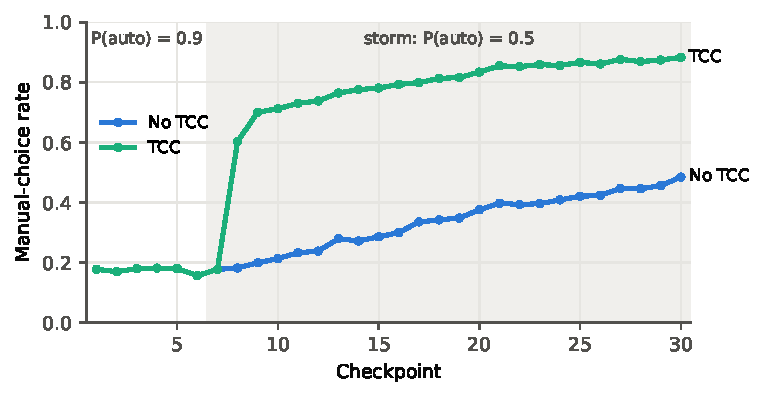
\includegraphics[width=0.72\linewidth]{fig1_reproduction_manual_rate.pdf}
\caption{Manual-choice rate per checkpoint. Before the storm the groups are identical (no TCCs fire); afterwards the TCC group switches to manual inspection within two checkpoints.}\label{fig:repro}
\end{figure}
Table~\ref{tab:repro} and Fig.~\ref{fig:repro} show the reproduction. No TCC fired in good weather (both groups: manual rate 0.174). In the storm phase the TCC group chose manual inspection far more often (0.779 vs.\ 0.335, $\Delta=+0.443$, $p<0.001$), which supports H1 and reproduces the original direction. Two discrepancies remain. First, the simulated no-TCC group also increased its manual rate ($+0.161$), whereas the original no-TCC group did not change; our simulated users learn from observed failures, whereas the original participants may have received less outcome feedback. Second, storm-phase accuracy was significantly higher with the TCC ($+0.106$, $p<0.001$), whereas the original found no significant difference (its TCC groups scored only numerically higher). Our simulation imposes no time cost on manual inspection, unlike the original's 8.5-minute limit, and has far more statistical power. We therefore accept the re-implementation as a faithful model of the \emph{mechanism} and use it as baseline B2, without claiming to reproduce human effect sizes.

\subsection{RQ2: Main comparison}
\begin{table}[!htbp]\centering\small
\caption{Part 2 results, mean over 50 seeds. Cost = decision cost per claim; AppRel = appropriate reliance; AccErr = accepted wrong claims / $N$; UnnVer = needless verifications / $N$; VE = verification efficiency.}\label{tab:main}
\begin{tabular}{lrrrrrr}
\toprule
Condition & Cost$\downarrow$ & $E_{trust}\downarrow$ & AppRel$\uparrow$ & AccErr$\downarrow$ & UnnVer$\downarrow$ & VE$\uparrow$ \\
\midrule
B0 No cue & 1.120 & 0.166 & 0.499 & 0.117 & 0.274 & 0.241 \\
B1 Reliability display & 1.105 & 0.157 & 0.499 & 0.103 & 0.302 & 0.242 \\
B2 Adaptive TCC & 1.062 & 0.170 & 0.507 & 0.077 & 0.340 & 0.251 \\
\textbf{Evidence-aware} & 0.999 & 0.124 & 0.597 & 0.080 & 0.257 & 0.278 \\
\midrule
Ablation: stage-only & 1.049 & 0.141 & 0.554 & 0.093 & 0.270 & 0.263 \\
Ablation: evidence-only & 1.053 & 0.143 & 0.546 & 0.091 & 0.283 & 0.259 \\
\midrule
\textit{Oracle (bound)} & 0.814 & 0.000 & 0.820 & 0.059 & 0.106 & 0.364 \\
\bottomrule
\end{tabular}
\end{table}
\begin{table}[!htbp]\centering\small
\caption{Paired differences, evidence-aware minus comparator (negative is better for Cost, $E_{trust}$, AccErr and UnnVer; positive is better for AppRel). 50 seeds; 95\% bootstrap CI; Holm-corrected Wilcoxon $p$.}\label{tab:comp}
\begin{tabular}{llrrrr}
\toprule
Metric & vs. & $\Delta$ mean & 95\% CI & $r_{rb}$ & $p_{Holm}$ \\
\midrule
Cost & B0 No cue & -0.1211 & [-0.1439, -0.1005] & -1.00 & $<$0.001 \\
Cost & B1 Reliability display & -0.1055 & [-0.1264, -0.0859] & -0.99 & $<$0.001 \\
Cost & B2 Adaptive TCC & -0.0631 & [-0.0801, -0.0465] & -0.87 & $<$0.001 \\
$E_{trust}$ & B0 No cue & -0.0415 & [-0.0450, -0.0380] & -1.00 & $<$0.001 \\
$E_{trust}$ & B1 Reliability display & -0.0328 & [-0.0361, -0.0296] & -1.00 & $<$0.001 \\
$E_{trust}$ & B2 Adaptive TCC & -0.0455 & [-0.0493, -0.0417] & -1.00 & $<$0.001 \\
AppRel & B0 No cue & +0.0977 & [+0.0877, +0.1079] & +1.00 & $<$0.001 \\
AppRel & B1 Reliability display & +0.0983 & [+0.0885, +0.1083] & +1.00 & $<$0.001 \\
AppRel & B2 Adaptive TCC & +0.0901 & [+0.0789, +0.1015] & +1.00 & $<$0.001 \\
AccErr & B0 No cue & -0.0372 & [-0.0445, -0.0305] & -1.00 & $<$0.001 \\
AccErr & B1 Reliability display & -0.0229 & [-0.0289, -0.0170] & -0.90 & $<$0.001 \\
AccErr & B2 Adaptive TCC & +0.0025 & [-0.0023, +0.0073] & +0.22 & 0.183 \\
UnnVer & B0 No cue & -0.0164 & [-0.0253, -0.0071] & -0.52 & 0.002 \\
UnnVer & B1 Reliability display & -0.0446 & [-0.0541, -0.0352] & -0.96 & $<$0.001 \\
UnnVer & B2 Adaptive TCC & -0.0829 & [-0.0918, -0.0744] & -1.00 & $<$0.001 \\
Cost & Ablation: stage-only & -0.0497 & [-0.0621, -0.0371] & -0.88 & $<$0.001 \\
Cost & Ablation: evidence-only & -0.0540 & [-0.0666, -0.0417] & -0.95 & $<$0.001 \\
$E_{trust}$ & Ablation: stage-only & -0.0174 & [-0.0193, -0.0155] & -1.00 & $<$0.001 \\
$E_{trust}$ & Ablation: evidence-only & -0.0189 & [-0.0211, -0.0167] & -1.00 & $<$0.001 \\
\bottomrule
\end{tabular}
\end{table}
\begin{figure}[!htbp]\centering
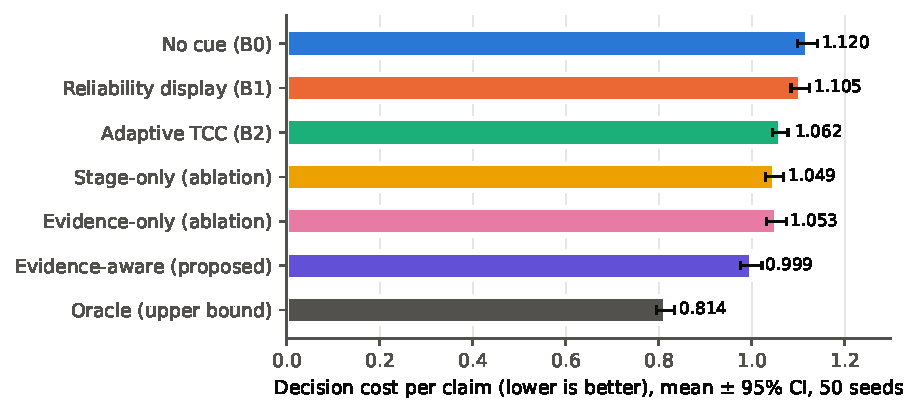
\includegraphics[width=0.72\linewidth]{fig2_main_decision_cost.pdf}\\[2pt]
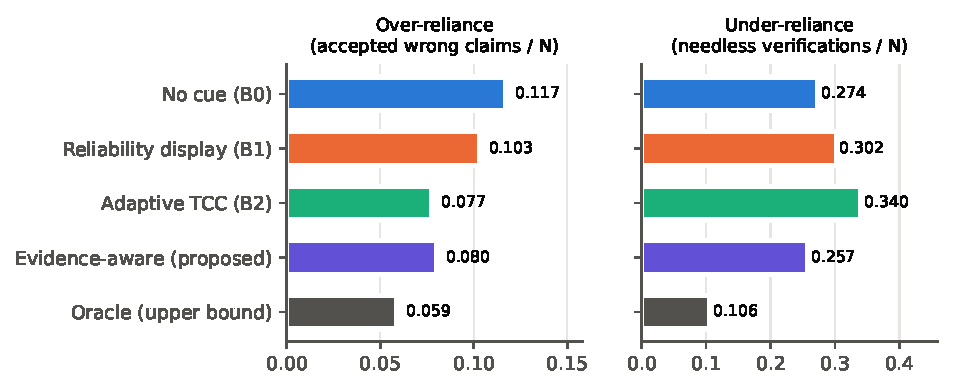
\includegraphics[width=0.78\linewidth]{fig3_reliance_decomposition.pdf}
\caption{Top: decision cost (mean $\pm$ 95\% CI). Bottom: decomposition into over-reliance (accepted wrong claims) and under-reliance (needless verifications).}\label{fig:main}
\end{figure}
The evidence-aware cue had the lowest decision cost of all non-oracle conditions (0.999; Table~\ref{tab:main}, Fig.~\ref{fig:main}). Relative to B0, B1 and B2 the paired reductions were $-0.121$, $-0.106$ and $-0.063$ (all $p_{Holm}<0.001$; Table~\ref{tab:comp}), i.e.\ 10.8\%, 9.6\% and 5.9\%. Cost was lower in 49/50 seeds against B0 and B1, and in 43/50 against B2 ($r_{rb}=-0.87$). It also reduced calibration error by 0.033--0.045, raised appropriate reliance from about 0.50 to 0.60, and gave the highest verification efficiency (0.278: more of the claims users chose to check were actually wrong). H2 is supported. The proposed cue nevertheless closed only 39.6\% of the cost gap between B0 and the oracle; the remainder reflects partial compliance and noisy user decisions.

\emph{The mechanism differs by comparator.} Against B0 and B1, the evidence-aware cue reduced both accepted errors and needless verifications. Against B2 it did \emph{not} reduce accepted errors ($+0.003$, CI $[-0.002, 0.007]$, $p=0.18$); its entire advantage came from 0.083 fewer needless verifications per claim. B2 already curbs over-trust effectively, but because it only ever pushes users towards verification, it produced the highest under-reliance of any condition (0.340).

\paragraph{Ablation.} Both components were needed: the full model beat stage-only by $-0.050$ and evidence-only by $-0.054$ in cost (both $p<0.001$), and each ablation still beat B0--B2 on cost (Table~\ref{tab:main}).

\subsection{RQ3: Robustness, sensitivity and drift}
\begin{table}[!htbp]\centering\small
\caption{Decision cost (mean over 50 seeds) under the deeper analyses. Bold = lowest mean among non-oracle conditions; Section~\ref{sec:rq3} reports which differences are significant. Stage = stage-only ablation; EA = evidence-aware.}\label{tab:analyses}
\begin{tabular}{lrrrrrr}
\toprule
Setting & B0 & B1 & B2 & Stage & \textbf{EA} & Oracle \\
\midrule
Noise SD = 0 & 1.120 & 1.105 & 1.062 & 1.049 & \textbf{0.997} & 0.814 \\
Noise SD = 0.1 & 1.120 & 1.105 & 1.062 & 1.049 & \textbf{0.999} & 0.814 \\
Noise SD = 0.2 & 1.120 & 1.105 & 1.062 & 1.049 & \textbf{1.010} & 0.814 \\
Noise SD = 0.35 & 1.120 & 1.105 & 1.062 & 1.049 & \textbf{1.022} & 0.814 \\
Noise SD = 0.5 & 1.120 & 1.105 & 1.062 & 1.049 & \textbf{1.029} & 0.814 \\
Compliance = 0.1 & 1.120 & 1.112 & 1.079 & 1.094 & \textbf{1.075} & 0.814 \\
Compliance = 0.3 & 1.120 & 1.106 & 1.074 & 1.078 & \textbf{1.039} & 0.814 \\
Compliance = 0.5 & 1.120 & 1.105 & 1.062 & 1.049 & \textbf{0.999} & 0.814 \\
Compliance = 0.7 & 1.120 & 1.099 & 1.056 & 1.022 & \textbf{0.962} & 0.814 \\
Compliance = 0.9 & 1.120 & 1.105 & 1.052 & 1.003 & \textbf{0.944} & 0.814 \\
Uninformative evidence ($\beta$=0) & 1.073 & 1.070 & 1.038 & 1.006 & \textbf{1.005} & 0.880 \\
Drift, pre-change & 1.120 & 1.116 & 1.076 & 1.067 & \textbf{1.030} & 0.809 \\
Drift, post-change & 1.203 & 1.169 & 1.120 & 1.070 & \textbf{1.027} & 0.847 \\
\bottomrule
\end{tabular}
\end{table}
\begin{figure}[!htbp]\centering
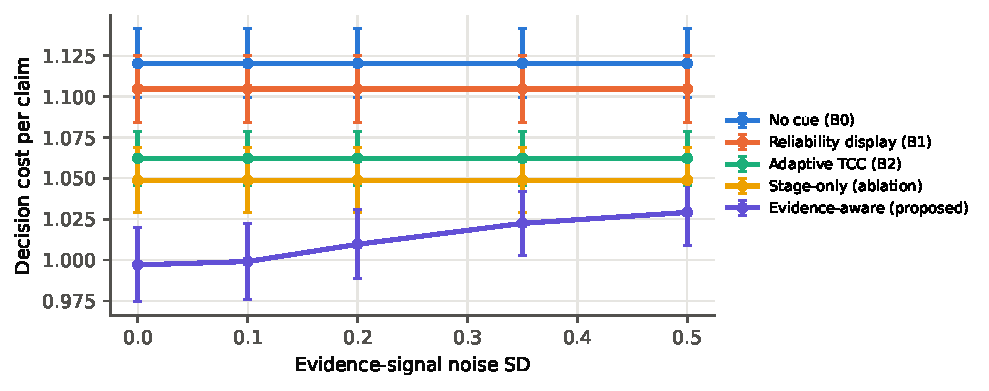
\includegraphics[width=0.66\linewidth]{fig4_noise_robustness.pdf}\\[2pt]
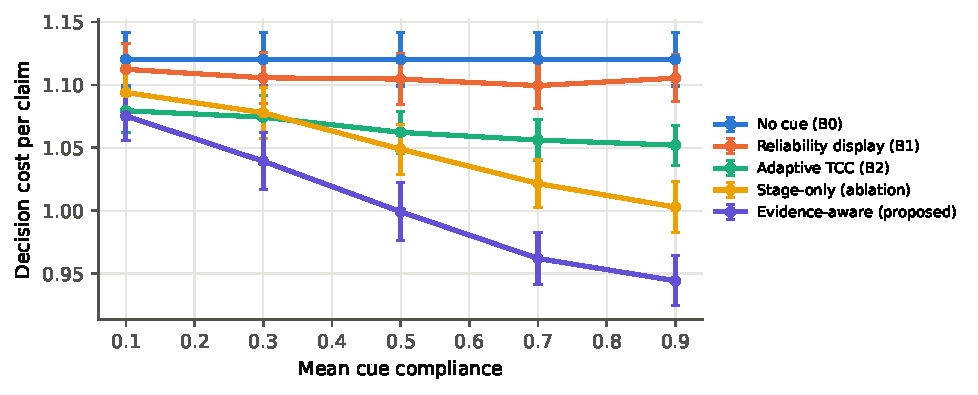
\includegraphics[width=0.66\linewidth]{fig5_compliance_sensitivity.pdf}\\[2pt]
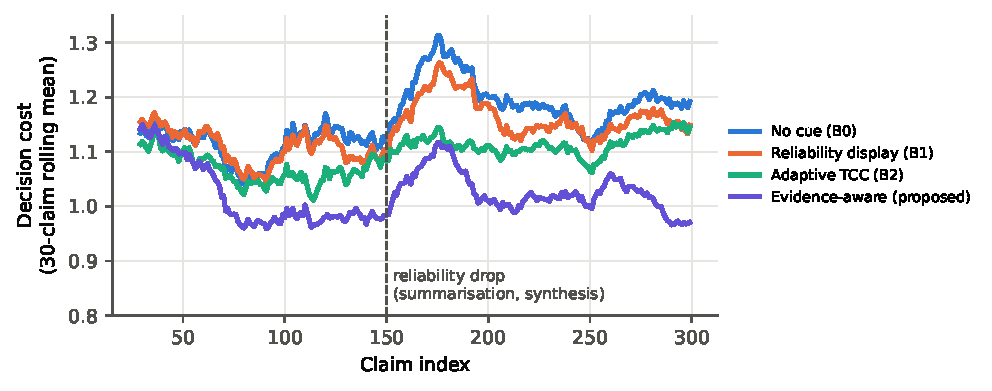
\includegraphics[width=0.66\linewidth]{fig6_drift.pdf}
\caption{Top: evidence-signal noise (A1). Middle: cue compliance (A3). Bottom: reliability drift after claim 150 (A4), shown as a 30-claim rolling mean averaged over seeds. Error bars are between-seed 95\% intervals; the paired tests in the text are more sensitive.}\label{fig:analyses}
\end{figure}
\label{sec:rq3}
\textbf{A1, noise.} As the evidence signal degraded (SD $0\to0.5$), the evidence-aware cost rose from 0.997 to 1.029, and its advantage over B2 shrank from $-0.065$ to $-0.033$ and over stage-only from $-0.052$ to $-0.020$. All differences remained significant ($p_{Holm}\le0.0003$).
\textbf{A2, uninformative evidence (negative control).} With $\beta=0$, the evidence-aware and stage-only cues were indistinguishable ($\Delta=-0.001$, CI $[-0.008,0.006]$, $p=0.56$): the model learned to ignore evidence and did no harm, so H3 is supported. It still beat B2 ($-0.034$), because stage-level reliability remained informative.
\textbf{A3, compliance.} The benefit depends on users acting on the cue. At mean compliance 0.1 the evidence-aware cue was no better than B2 ($\Delta=-0.004$, CI $[-0.017,0.008]$, $p=0.40$); at 0.9 it was $0.108$ better. B2 is comparatively insensitive to compliance because it fires rarely (16.5 times per 300 claims on average) and also lowers trust directly.
\textbf{A4, drift.} After the reliability drop, the evidence-aware cost was essentially unchanged (1.030 pre, 1.027 post), whereas B0 rose from 1.120 to 1.203 and B2 from 1.076 to 1.120. The post-change advantages were $-0.176$ (B0), $-0.143$ (B1), $-0.093$ (B2) and $-0.043$ (stage-only), all $p<0.001$. Online refitting tracks the change faster than users' experience-based trust does.

\subsection{Failure analysis (A5)}
\begin{figure}[!htbp]\centering
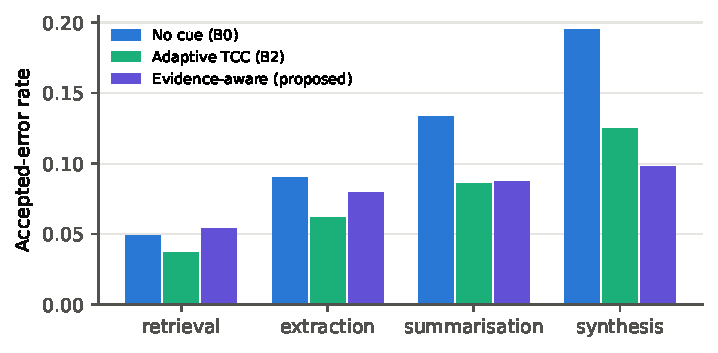
\includegraphics[width=0.62\linewidth]{fig7_failures_by_stage.pdf}
\caption{Accepted-error rate by pipeline stage. The evidence-aware cue helps most on synthesis but accepts \emph{more} wrong retrieval claims than both baselines.}\label{fig:fail}
\end{figure}
The gains are concentrated where they matter most. On synthesis claims, accepted errors fell from 0.195 (B0) and 0.125 (B2) to 0.098 (Fig.~\ref{fig:fail}). The cue has a clear failure mode, though. On highly reliable retrieval claims it \emph{raised} confidence and accepted more wrong claims (0.054) than B0 (0.049) or B2 (0.037), in exchange for far fewer needless verifications of retrieval claims (0.392 vs.\ 0.466 and 0.563). By evidence level, 87\% of the residual accepted errors under the evidence-aware cue occurred on low- or mid-evidence claims, where the warranted probability lies close to the decision threshold and the cue cannot separate the two cases.

\section{Discussion}
\paragraph{What the evidence supports.} In this simulation, separating ``how reliable is this stage'' from ``how well supported is this claim'' (the review's Eq.~7) improved calibration in a measurable way, and both terms contributed (ablation). The comparison with the adaptive TCC sharpens the picture. An over-trust detector such as the TCC is very good at preventing users from accepting wrong claims, but it pays for this with excess verification, a cost the review flagged as under-studied (its \S8.5). A per-claim cue can lower trust where evidence is weak \emph{and raise it where evidence is strong}. That two-sided adjustment is the source of its advantage, which matches the review's position that calibration, not maximal trust, is the goal.

\paragraph{What it does not support.} First, the advantage is conditional: it needs an informative evidence signal (A1, A2) and users who act on cues (A3). An evidence-aware interface whose users ignore it is no better than a TCC. Second, a two-sided cue can create over-reliance in exactly the places where the agent is usually right (A5, retrieval). A practical design might combine the evidence-aware display with an over-trust detector, a combination we did not test. Third, nothing here estimates effect sizes for real people.

\paragraph{Relation to the proposed framework.} The results give partial, simulation-level support for three components of the review's framework (evidence collection, trust-state estimation, adaptive communication) and for its emphasis on verification efficiency. They give no evidence about its human-state component, which we did not model.

\section{Threats to Validity and Limitations}
\textbf{External validity (main threat).} All users are simulated with a simple experience-based trust model; the absolute numbers mean nothing for humans, and some mechanisms, such as the absence of an R2 effect, may differ in people. \textbf{Construct validity.} The proposed estimator shares the logistic form of the generator, which favours it; A1 and A2 test noise and irrelevance but not misspecification. Stage reliabilities and the cost ratio $L/c=5$ are illustrative, not measured. \textbf{Internal validity.} Common random numbers, a frozen protocol, separate debugging seeds and logged protocol changes reduce the risk of tuning to the results. All analyses were pre-specified, but parameter ranges were chosen by the author. \textbf{Reproduction.} No official code was found; the TCC is re-implemented from the paper's text, and its modality is abstracted to a compliance probability. \textbf{Statistical.} With 50 seeds even small effects are significant; we therefore report effect sizes and confidence intervals, and interpret differences below about 0.01 cost as practically negligible.

\section{Conclusion}
We re-implemented and partially reproduced a published adaptive trust-calibration mechanism, then tested the evidence-aware calibration proposed in our earlier review against it in a simulated research pipeline with known ground truth. Per-claim, evidence-aware cues lowered decision cost and calibration error, mainly by reducing needless verification rather than accepted errors, and they did so only when the evidence signal was informative and users heeded the cue. The most valuable next step is a small human study on the same claim streams, followed by a misspecified-generator test and a combined evidence-aware + TCC condition.

\paragraph{Reproducibility.} Code, frozen configuration, logs, per-claim outputs and figure scripts are in the accompanying repository; \texttt{bash scripts/run\_all.sh} regenerates every number, table and figure in about 10 seconds on a CPU.

\paragraph{AI-use statement.} An AI assistant (Claude, Anthropic) was used to draft the simulation code, analysis scripts, documentation and this manuscript, and to execute the experiments. All reported numbers were produced by executed code, and the tables are generated from result files. AI-proposed claims were checked against sources and outputs; the cases where the assistant's own summaries were corrected are documented in \texttt{ai\_assistance\_log.md}. The author is responsible for the content.

\bibliographystyle{plainnat}
\bibliography{references}
\end{document}

